\documentclass[a4paper]{article}
\usepackage{graphicx}
\graphicspath{/home/angelo/Documents/Uni/Courses/Advanced Statistics and programming/Assignments/assignment2/} 
\usepackage{mathtools}
\usepackage[a4paper, total={5in, 6.5in}]{geometry}
\usepackage{color}
\usepackage{tikz}
\usepackage{lipsum}
\usepackage{geometry}
\geometry{a4paper, left=2.5cm, top=2.5cm, bottom=2.5cm, right=2.5cm}
\usepackage{changepage}
\usepackage{booktabs}
\usepackage[font=small]{caption}
\DeclareCaptionFormat{mycaptionfont}{\fontsize{12}{13}\selectfont#1#2#3}
\usepackage{threeparttable}
\usepackage{ntheorem}
\usepackage{caption}
\usepackage{wrapfig,lipsum,booktabs}
\usepackage{listings}
\usepackage{pdflscape}
\captionsetup{format=mycaptionfont}
\usepackage{subcaption}
\theoremseparator{:}
\usepackage{lscape}

\usepackage[utf8]{inputenc}
\newtheorem{hyp}{Hypothesis}
\usetikzlibrary{shapes,decorations,arrows,calc,arrows.meta,fit,positioning}
\tikzset{
    -Latex,auto,node distance =1 cm and 1 cm,semithick,
    state/.style ={ellipse, draw, minimum width = 0.7 cm},
    point/.style = {circle, draw, inner sep=0.04cm,fill,node contents={}},
    bidirected/.style={Latex-Latex,dashed},
    el/.style = {inner sep=2pt, align=left, sloped}
}





\begin{document}

\title{ASAP Assignment 2}
\author{Angelo Barisano; 508903 }
\date{September 23rd, 2022}
\maketitle

\newpage
\section{Difference in Difference}


Description:
You are tasked with estimating the effects of the 1993 policy intervention on labor supply for single women by whether or not they had children.
--> The relevant varibales in this case are: 
state - US-State/ provice of residence
year - Year
urate - US-State/province unemployment rate
children - number of children per women
nonwhite - nonwhite
finc - annual family income
earn - anual earnings (of women)
age - age of women
ed - Years of education
work - Indicator work status (employed or not)
unearn - unearn Income 

Outcome variable: INDICATOR WORK STATUS
Time indicator: at 1993 (beginning) create time variable
Goal: estimate the effect of the 1993 policy intervention on labor supply for single women by whether or not they had children (Dummy for whether they had children or not??)


The unit of analysis are females in the US

Question: The main predictor is meant to be whether women has children; Should we use that as a dummy or numeric variable?? --> something like degree of treatment



\subsection{Indicate which of the coefficients(s) from equation (1) yield the following outcomes}

SEE SLIDE 57 ff

Important: we canot identify the monthrs; so If they become mothers at some point, we will assume that these are taken out!



$
(1) {y_{it}} = \beta_{0} + \beta_{1} + \beta_{2} + \beta_{3} D_i T_t + \epsilon_{it}
$


$E = (y_{T=1} | D=1)$
$E = (y_{T=0} | D=1)$
$E = (y_{T=1} | D=0)$
$E = (y_{T=0} | D=0)$

$
[E(y_{T=1} | D=1) - E(y_{T=0} | D=1)] - [E(y_{T=1} | D=0) - E(y_{T=0} | D=0)]
$




\subsection{Task 2: Provide a suiatble matrix plot as on slide 55}


\begin{wrapfigure}{L}{8.5cm}
\centering
\begin{subfigure}[b]{0.55\textwidth}
    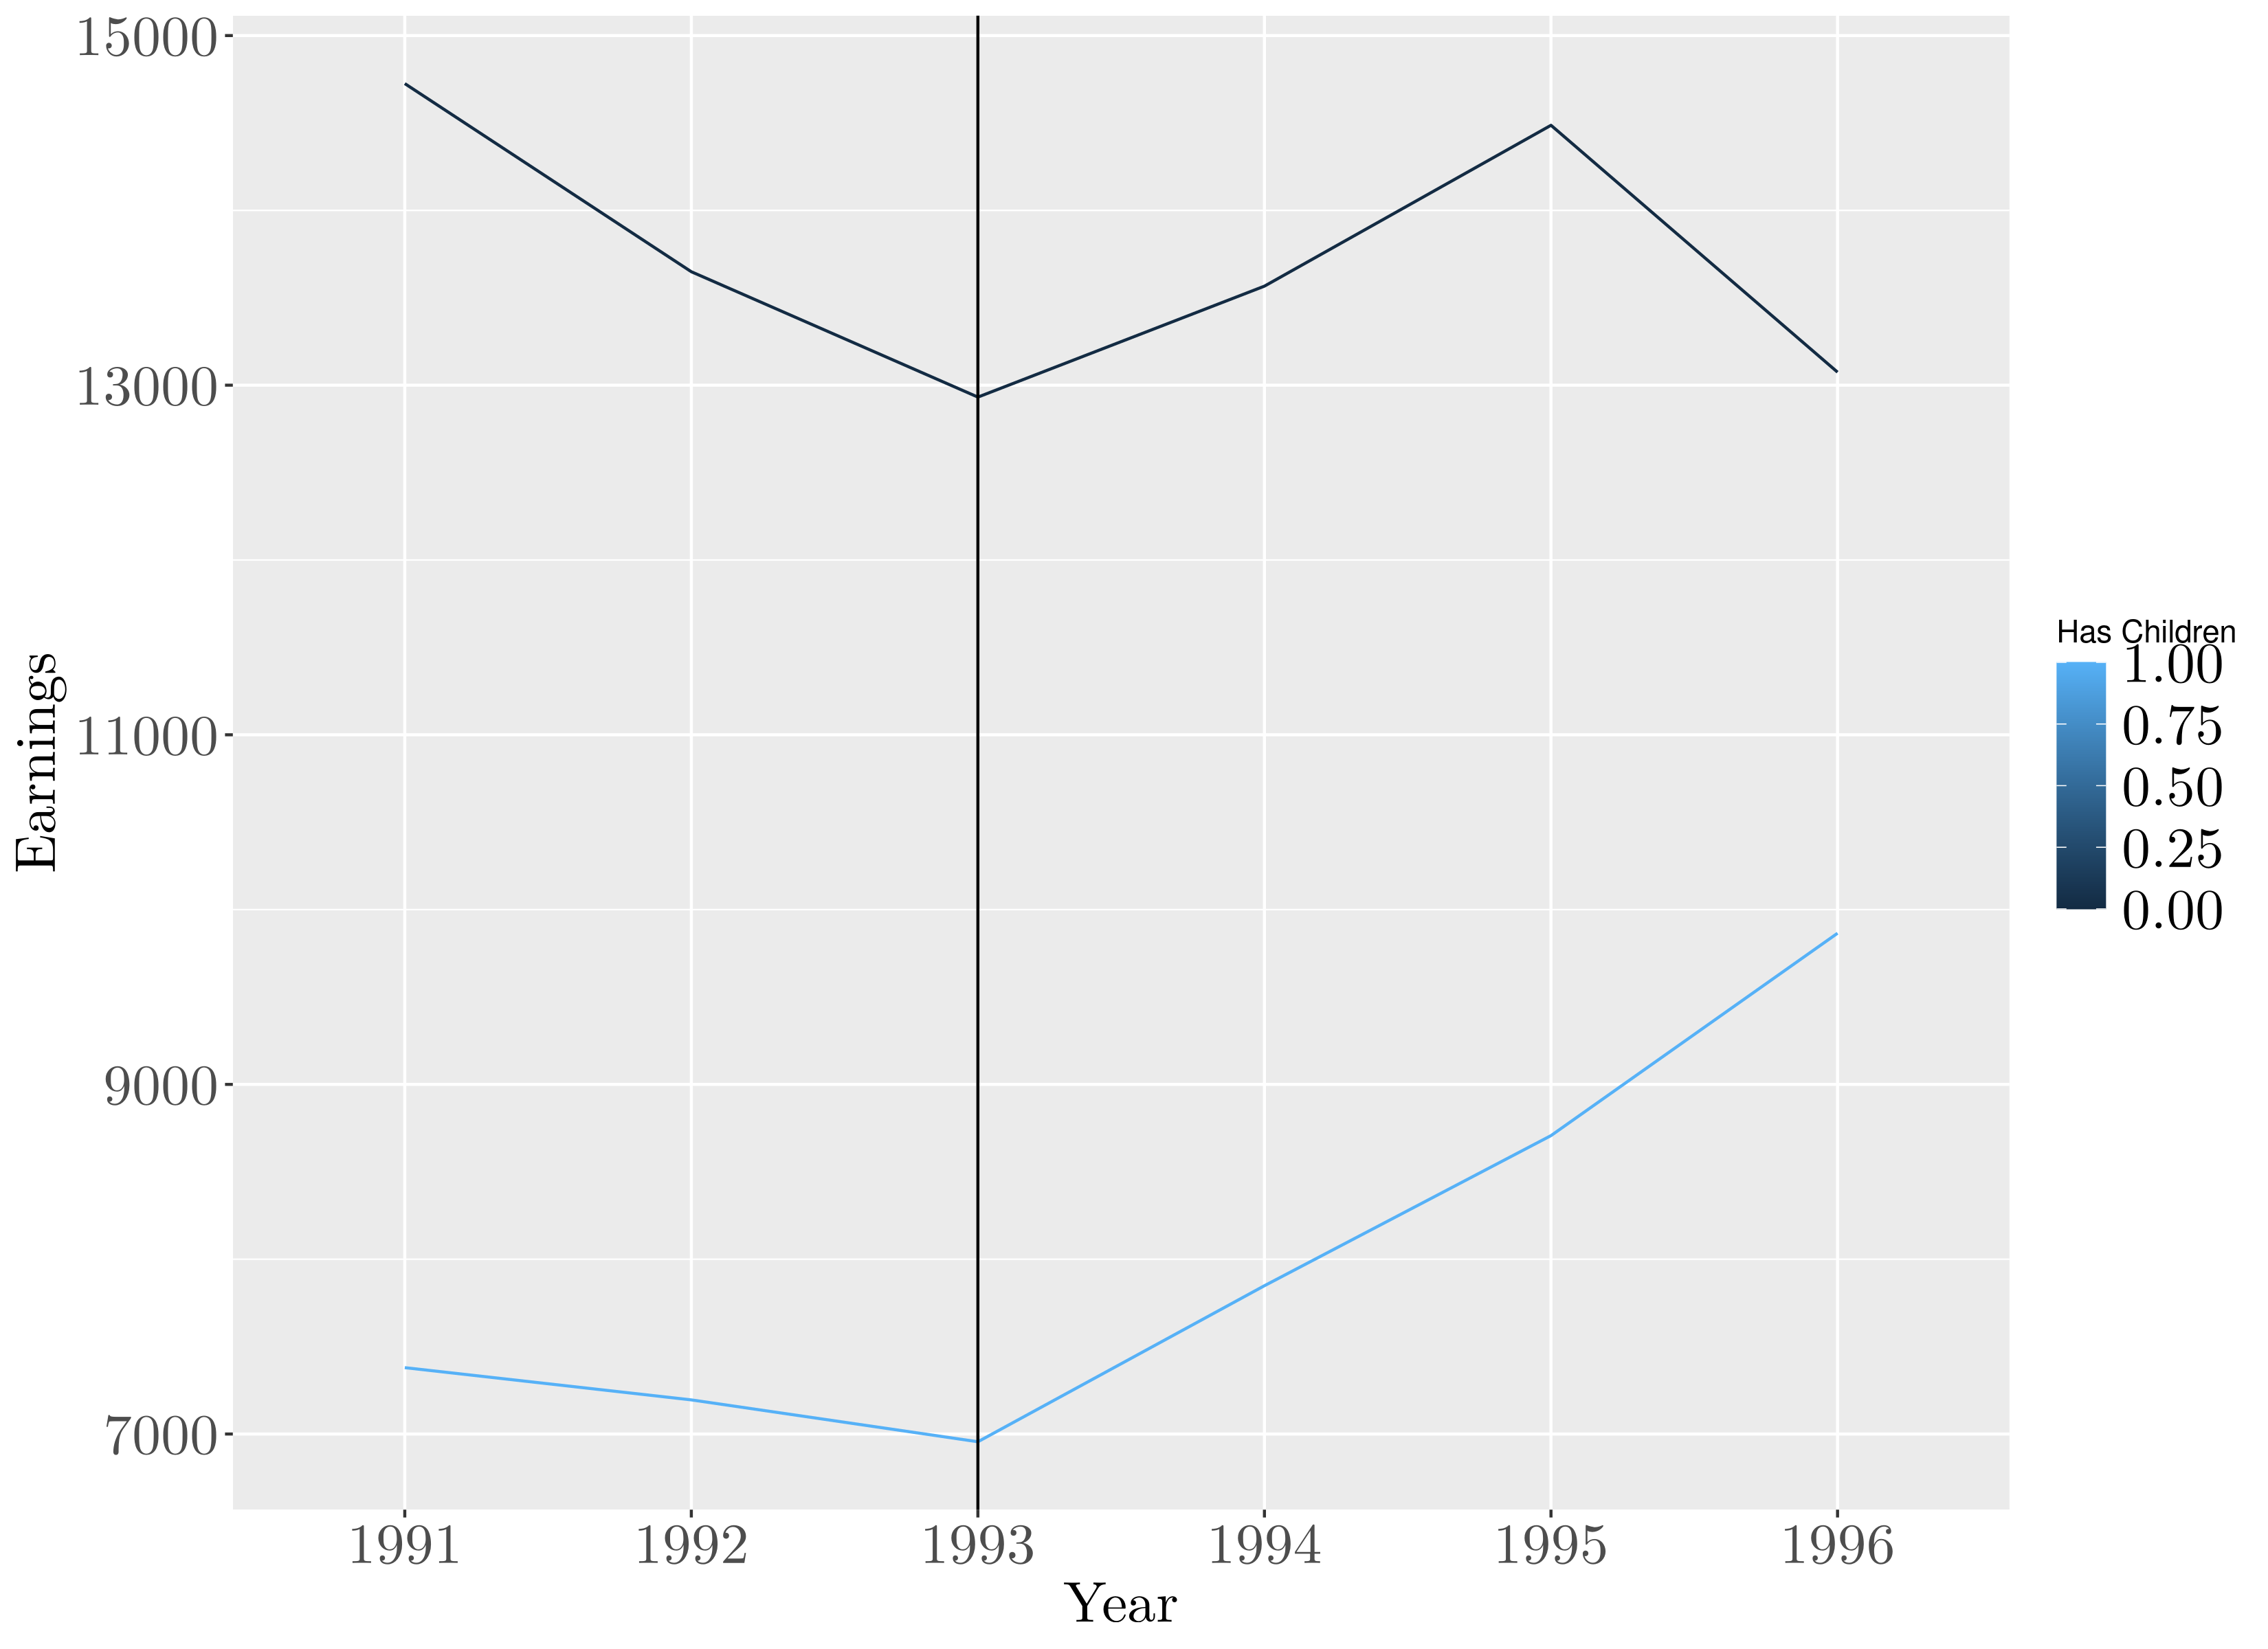
\includegraphics[width=.95\linewidth]{"/home/angelo/Documents/Uni/Courses/Advanced Statistics and programming/Assignments/assignment2/Graphics/task2_earn_did.png"} 
   \caption{Annual Earnings by Females with(out) Children}
   \label{fig:Ng2}
\end{subfigure}

\begin{subfigure}[b]{0.55\textwidth}
    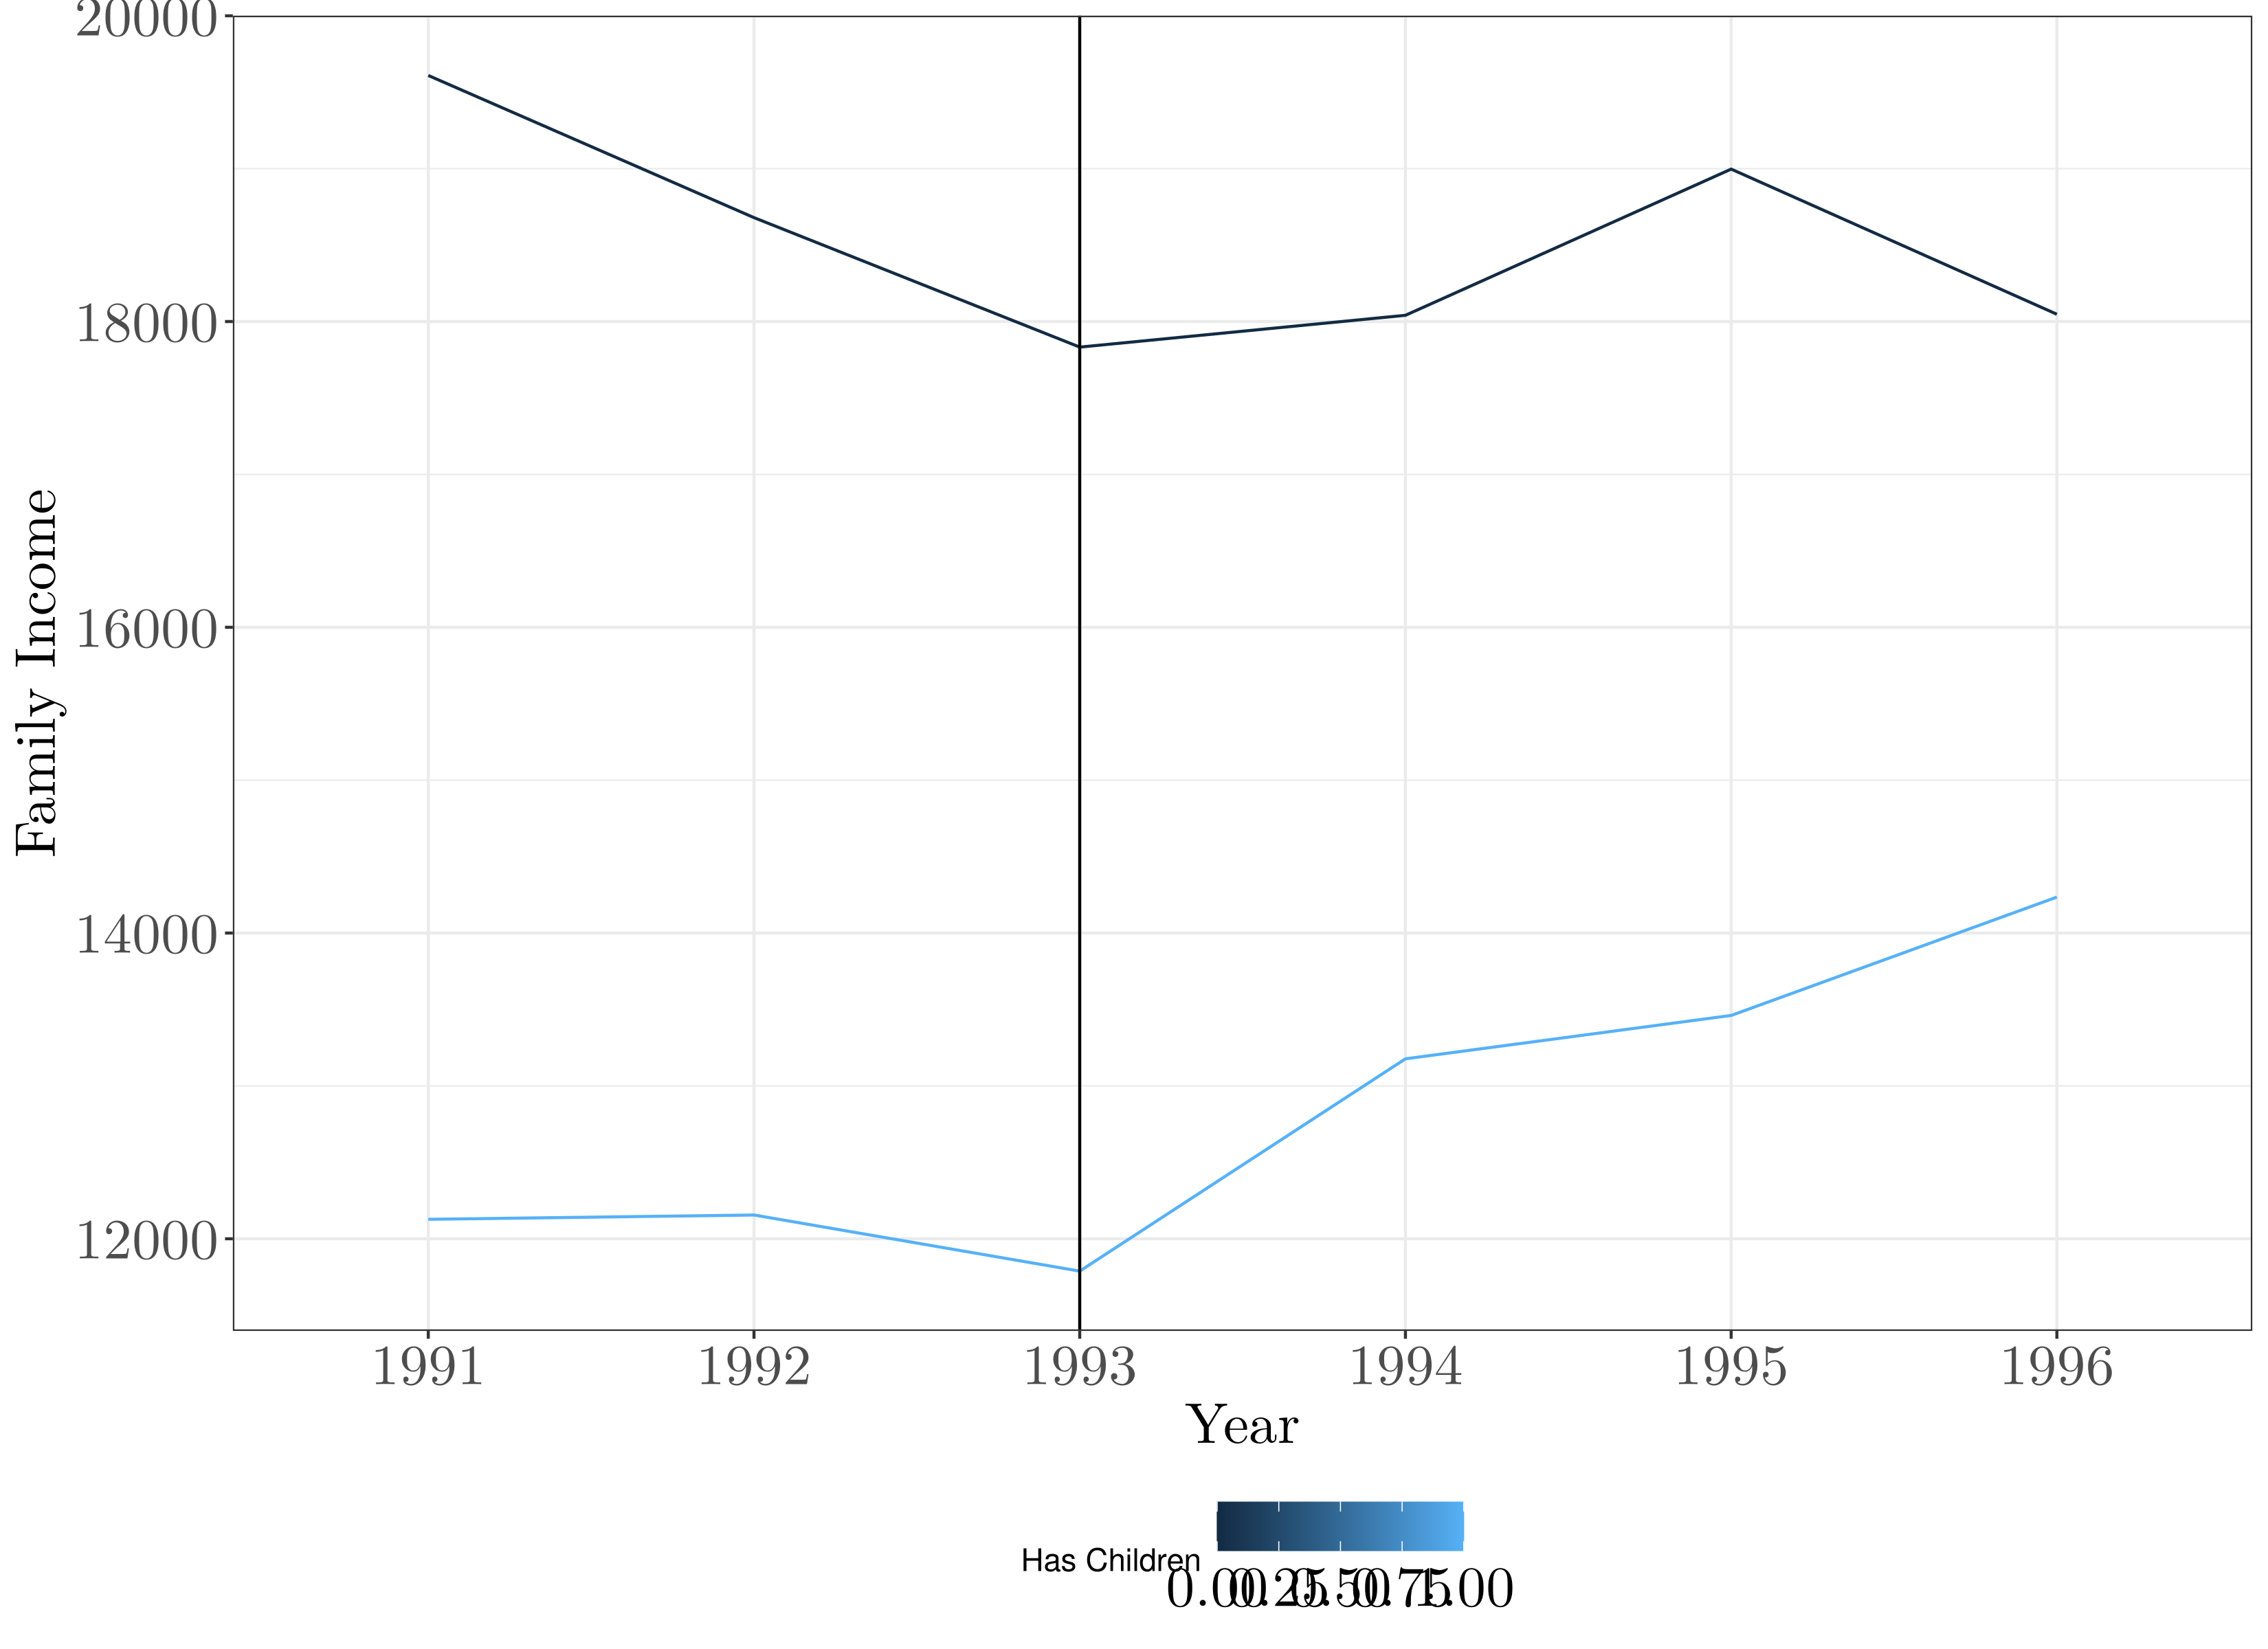
\includegraphics[width=.95\linewidth]{"/home/angelo/Documents/Uni/Courses/Advanced Statistics and programming/Assignments/assignment2/Graphics/task2_finc_did.png"} 
   \caption{Family Earnings Earnings by Females with(out) Children}
   \label{fig:Ng2}
\end{subfigure}

\begin{subfigure}[b]{0.55\textwidth}
    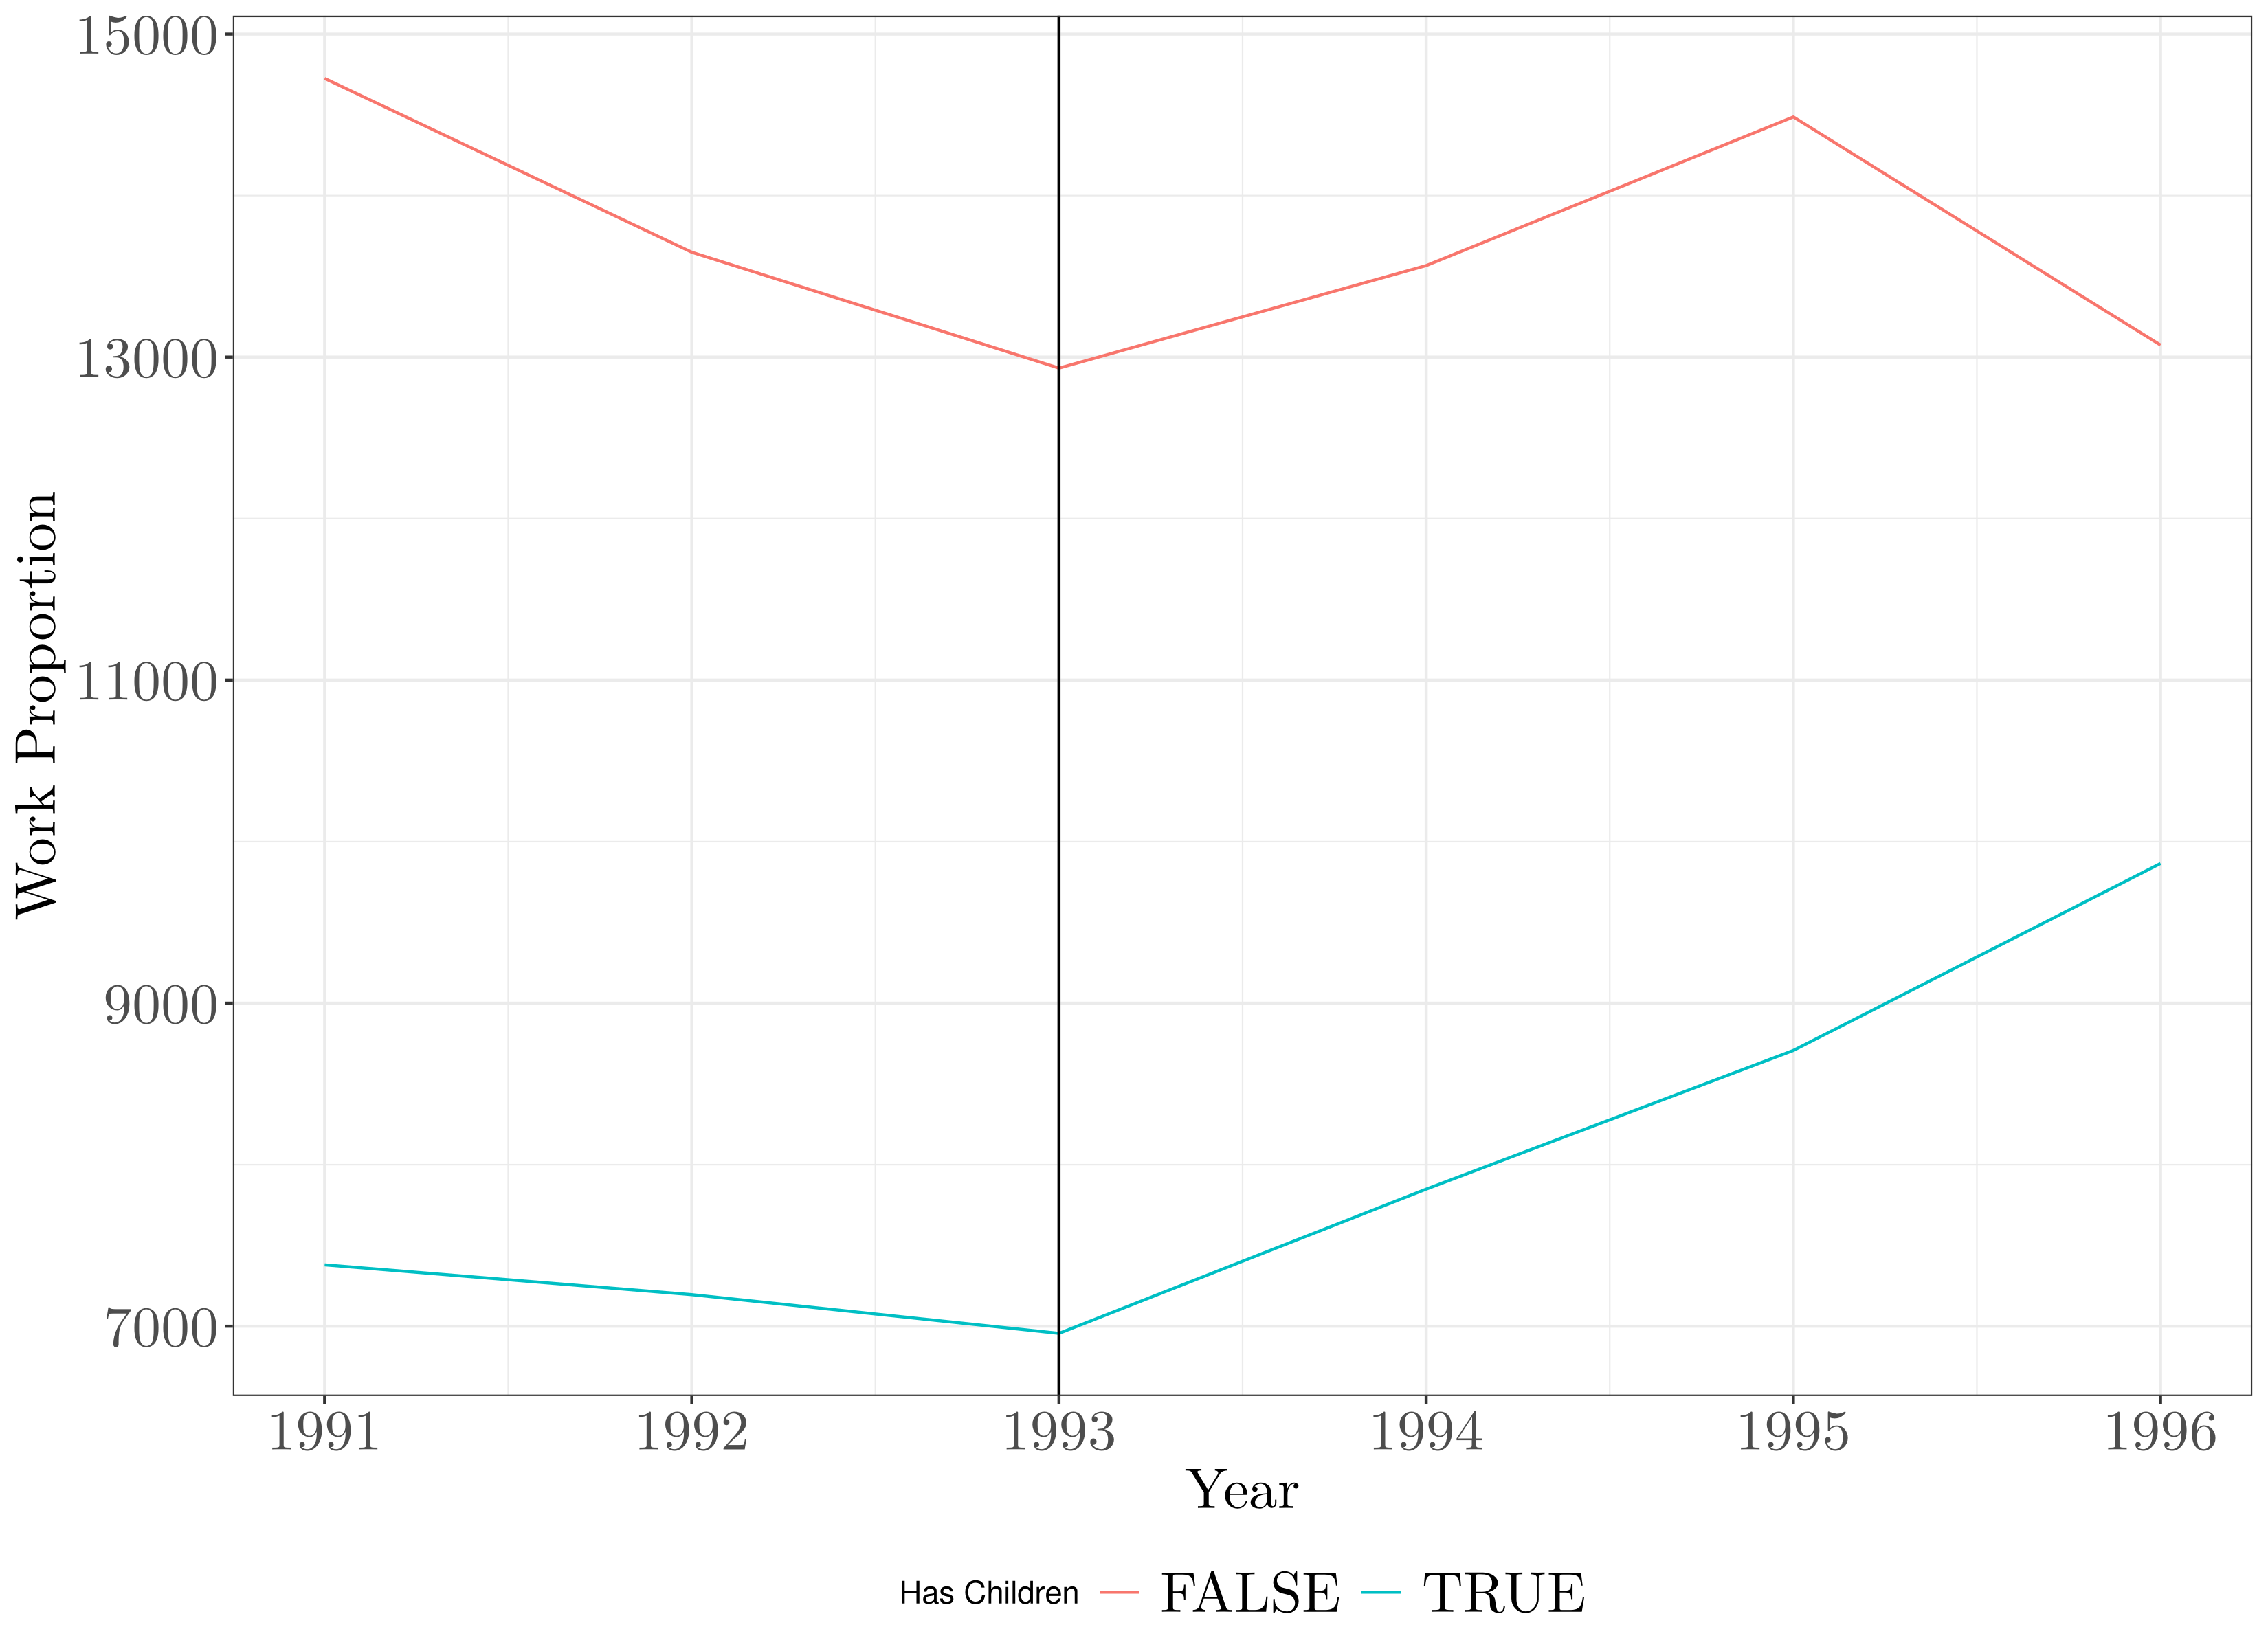
\includegraphics[width=.95\linewidth]{"/home/angelo/Documents/Uni/Courses/Advanced Statistics and programming/Assignments/assignment2/Graphics/task2_work_did.png"}  
   \caption{Work Participation by Females with(out) Children}
   \label{fig:Ng2}
\end{subfigure}
\captionsetup{justification=centering}
\caption{Pre-Post Intervention of EICT Credit for Women with(out) Children}
\end{wrapfigure}





NOTES: This "visoual" proof is no real proove; this is just visual confirmation of what we assume; but does this really pertain to the case that the TAX credit is the real cause? What about the case of subsections of the population? and we still do not know whether this is really causal and not like the economy heating up!`
Predictor is WHETHER YOU HAVE CHILD OR NOT


\subsection{Task 3: Summary Statistics for data}

% Table created by stargazer v.5.2.3 by Marek Hlavac, Social Policy Institute. E-mail: marek.hlavac at gmail.com
% Date and time: Fri, Sep 23, 2022 - 20:25:57
\begin{table}[!htbp] 
\begin{adjustwidth}{-0cm}{-0cm}
\begin{threeparttable}
\small
\captionsetup{font=small, justification=raggedright,singlelinecheck=false}
  \caption{Descriptive Statistics of Numeric Indepdenent and Dependent Varaible} 
  \label{} 
\begin{tabular}{@{\extracolsep{5pt}}lccccccc} 
\\[-1.8ex]\hline 
\hline \\[-1.8ex] 
Statistic & \multicolumn{1}{c}{Mean} & \multicolumn{1}{c}{St. Dev.} & \multicolumn{1}{c}{Min} & \multicolumn{1}{c}{Pctl(25)} & \multicolumn{1}{c}{Median} & \multicolumn{1}{c}{Pctl(75)} & \multicolumn{1}{c}{Max} \\ 
\hline \\[-1.8ex] 
Family Income & 15,255.320 & 19,444.250 & 0.000 & 5,123.418 & 9,636.664 & 18,659.180 & 575,616.800 \\ 
Earnings & 10,432.480 & 18,200.760 & 0.000 & 0.000 & 3,332.180 & 14,321.220 & 537,880.600 \\ 
Age & 35.210 & 10.157 & 20 & 26 & 34 & 44 & 54 \\ 
Education & 8.806 & 2.636 & 0 & 7 & 10 & 11 & 11 \\ 
Education Years & 4.823 & 7.123 & 0.000 & 0.000 & 2.973 & 6.864 & 134.058 \\ 
Unearned Income & 1.193 & 1.382 & 0 & 0 & 1 & 2 & 9 \\ 
Count Children & 0.513 & 0.500 & 0 & 0 & 1 & 1 & 1 \\ 
\hline \\[-1.8ex] 
\end{tabular} 
\begin{tablenotes}[para,flushleft]
      \small
      \item\textit{Notes:} N = 13746
    \end{tablenotes}
\end{threeparttable}
\end{adjustwidth}
\end{table}


% Table created by stargazer v.5.2.3 by Marek Hlavac, Social Policy Institute. E-mail: marek.hlavac at gmail.com
% Date and time: Fri, Sep 23, 2022 - 20:47:48
\begin{table}[!htbp] 
\begin{adjustwidth}{-0cm}{-0cm}
\begin{threeparttable}
\small
\captionsetup{font=small, justification=raggedright,singlelinecheck=false}
  \caption{Descriptive Statistics of ECIC; With Children} 
  \label{} 
\begin{tabular}{@{\extracolsep{5pt}}lccccccc} 
\\[-1.8ex]\hline 
\hline \\[-1.8ex] 
Statistic & \multicolumn{1}{c}{Mean} & \multicolumn{1}{c}{St. Dev.} & \multicolumn{1}{c}{Min} & \multicolumn{1}{c}{Pctl(25)} & \multicolumn{1}{c}{Median} & \multicolumn{1}{c}{Pctl(75)} & \multicolumn{1}{c}{Max} \\ 
\hline \\[-1.8ex] 
Family Income & 12,750.390 & 15,739.050 & 0.000 & 4,652.465 & 8,425.197 & 15,218.720 & 410,507.600 \\ 
Earnings & 7,909.934 & 14,956.930 & 0.000 & 0.000 & 1,110.727 & 11,107.270 & 366,095.500 \\ 
Age & 32.717 & 8.630 & 20 & 25 & 32 & 39 & 54 \\ 
Education & 9.001 & 2.408 & 0 & 7 & 10 & 11 & 11 \\ 
Education Years & 4.840 & 5.872 & 0.000 & 0.071 & 3.761 & 7.070 & 102.958 \\ 
Unearned Income & 2.097 & 1.209 & 1 & 1 & 2 & 3 & 9 \\ 
Count Children & 0.466 & 0.499 & 0 & 0 & 0 & 1 & 1 \\ 
\hline \\[-1.8ex] 
\end{tabular} 
\begin{tablenotes}[para,flushleft]
      \small
      \item\textit{Notes:} N = 7819
    \end{tablenotes}
\end{threeparttable}
\end{adjustwidth}
\end{table} 




% Table created by stargazer v.5.2.3 by Marek Hlavac, Social Policy Institute. E-mail: marek.hlavac at gmail.com
% Date and time: Fri, Sep 23, 2022 - 20:47:48
\begin{table}[!htbp] 
\begin{adjustwidth}{-0cm}{-0cm}
\begin{threeparttable}
\small
\captionsetup{font=small, justification=raggedright,singlelinecheck=false}
  \caption{Descriptive Statistics of ECIC; Without Children} 
  \label{} 
\begin{tabular}{@{\extracolsep{5pt}}lccccccc} 
\\[-1.8ex]\hline 
\hline \\[-1.8ex] 
Statistic & \multicolumn{1}{c}{Mean} & \multicolumn{1}{c}{St. Dev.} & \multicolumn{1}{c}{Min} & \multicolumn{1}{c}{Pctl(25)} & \multicolumn{1}{c}{Median} & \multicolumn{1}{c}{Pctl(75)} & \multicolumn{1}{c}{Max} \\ 
\hline \\[-1.8ex] 
Family Income & 18,559.860 & 23,041.780 & 0.000 & 5,793.092 & 11,912.950 & 24,391.010 & 575,616.800 \\ 
Earnings & 13,760.260 & 21,301.400 & 0.000 & 0.000 & 7,664.014 & 19,447.610 & 537,880.600 \\ 
Age & 38.498 & 11.046 & 20 & 28 & 40 & 49 & 54 \\ 
Education & 8.549 & 2.889 & 0 & 7 & 10 & 11 & 11 \\ 
Education Years & 4.800 & 8.496 & 0.000 & 0.000 & 1.248 & 6.528 & 134.058 \\ 
Unearned Income & 0.000 & 0.000 & 0 & 0 & 0 & 0 & 0 \\ 
Count Children & 0.574 & 0.494 & 0 & 0 & 1 & 1 & 1 \\ 
\hline \\[-1.8ex] 
\end{tabular} 
\begin{tablenotes}[para,flushleft]
      \small
      \item\textit{Notes:} N = 5927
    \end{tablenotes}
\end{threeparttable}
\end{adjustwidth}
\end{table}


\subsection{Task 4: Matrix Diff in Diff}
NOte: by taking the average of the periods we have two small problems: 1) the AFTER period is longer; so should we really do that?






\end{document}
